\documentclass[12pt, letterpaper]{article}
\usepackage[utf8]{inputenc}
\usepackage{amsmath, amsfonts, amssymb}
\usepackage{geometry}
\usepackage{graphicx}
\usepackage{fancyhdr}
\usepackage{pgfplots}
\usepackage{float}
\usepackage{pgfplotstable}
\usepackage{booktabs} 
\pgfplotsset{compat=1.18}

% Setup for homework style
\geometry{margin=1in}
\pagestyle{fancy}
\fancyhf{}
\lhead{APPM 2360: Differential Equations}
\rhead{Homework 2}
\cfoot{\thepage}

\title{Homework 2}
\author{Zachariah Galdston}
\date{9/5/2024}

\begin{document}

\maketitle

\section*{Problem 1}
\textbf{Problem Statement:} Consider the autonomous ODE $y' = 2y - y^2$


\subsection*{Part (a)}
\textbf{Problem Statement:} Find the equilibria.

\textbf{Solution:} To find the equilibrium solutions, we set the derivative equal to zero:

\[
2y - y^2 = 0
\]

Factorizing the equation:

\[
y(2 - y) = 0
\]

Thus, the equilibrium solutions are:

\[
y = 0 \quad \text{or} \quad y = 2
\]
\textbf{Problem Statement:} Determine the stability at each of equilibrium point

\textbf{Solution:} Solve for the sign of the derivative \( y' = 2y - y^2 \).

1. For \( y = 0 \): 
    \[
    \frac{dy}{dt} = 2y - y^2 = 2(0) - (0)^2 = 0
    \]
    Consider \( \frac{dy}{dt} \) near \( y = 0 \). For \( y > 0 \), \( 2y - y^2 > 0 \), meaning the solution increases, and for \( y < 0 \), \( 2y - y^2 < 0 \), meaning the solution decreases. Hence, \( y = 0 \) is unstable.
\hfill \break

    2. For \( y = 2 \):
    \[
    \frac{dy}{dt} = 2(2) - (2)^2 = 4 - 4 = 0
    \]
    Consider \( \frac{dy}{dt} \) near \( y = 2 \). For \( y > 2 \), \( 2y - y^2 < 0 \), meaning the solution decreases, and for \( y < 2 \), \( 2y - y^2 > 0 \), meaning the solution increases. Hence, \( y = 2 \) is stable.
\subsection*{Part (b)}
\textbf{Problem Statement:} Sketch the direction field and solution through $(0,1)$.
\begin{figure}[h!]
    \centering
    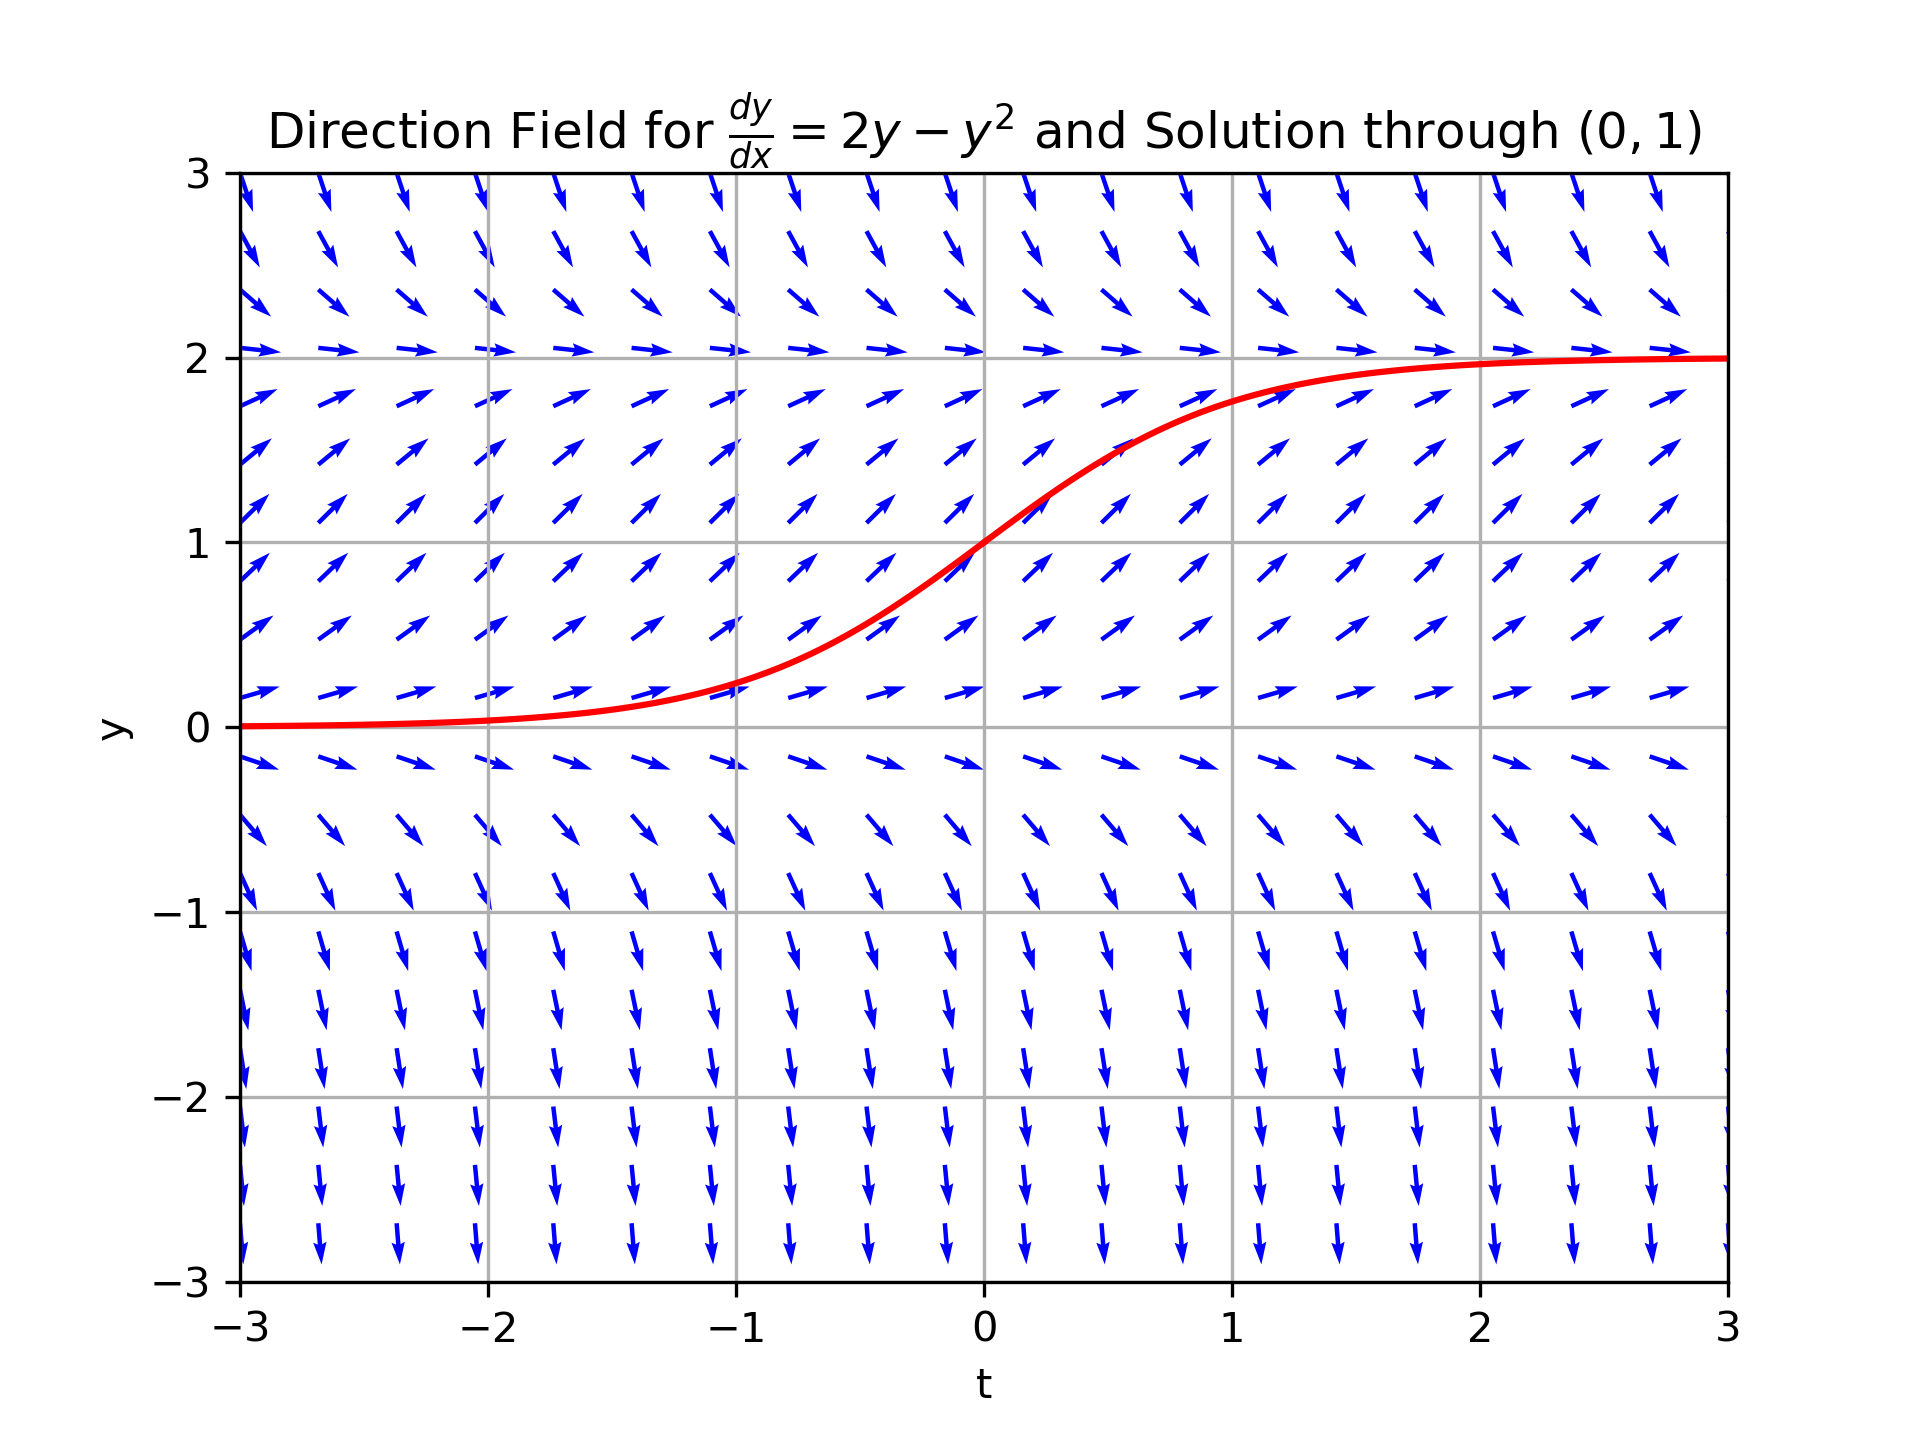
\includegraphics[width=0.8\textwidth]{direction_field_solution.png} % Adjust the filename/path accordingly
    \caption{Direction Field and Solution passing through $(0,1)$}
    \label{fig:direction_field}
\end{figure}
\subsection*{Part (c)}
\textbf{Problem Statement:} Describe the long term behavior.

(i) For the initial point \( (-1, 3) \), the solution approaches \( y = 2 \) as \( t \to \infty \), since \( y = 2 \) is a stable equilibrium and the initial value of \( y = 3 \) is greater than 2.

(ii) For the initial point \( (0, -1) \), since \( y = 0 \) is an unstable equilibrium, the solution decreases indefinitely as \( t \to \infty \).

\subsection*{Part (d)}
\textbf{Problem Statement:} Find the general solution.

\textbf{Solution:}The differential equation can be rewritten as:

\[
\frac{dy}{dt} = 2y - y^2
\]

This is separable. We rewrite it as:

\[
\frac{1}{y(2 - y)} dy = dt
\]

Using partial fraction decomposition:

\[
\frac{1}{y(2 - y)} = \frac{A}{y} + \frac{B}{2 - y}
\]

Multiplying both sides by \( y(2 - y) \), we get:

\[
1 = A(2 - y) + By
\]

Equating coefficients:

\[
A = \frac{1}{2}, \quad B = \frac{1}{2}
\]

Thus, the equation becomes:

\[
\frac{1}{2} \left( \frac{1}{y} + \frac{1}{2 - y} \right) dy = dt
\]

Integrating both sides:

\[
\frac{1}{2} \left( \ln |y| - \ln |2 - y| \right) = t + C
\]

Simplifying:

\[
\ln \left( \frac{y}{2 - y} \right) = 2t + C
\]

Exponentiating both sides:

\[
\frac{y}{2 - y} = e^{2t + C}
\]

Let \( C = e^{C} \), then:

\[
\frac{y}{2 - y} = C e^{2t}
\]

Solving for \( y \):

\[
y = \frac{2C e^{2t}}{1 + C e^{2t}}
\]

\subsection*{Part (e)}
\textbf{Problem Statement:} Find particular solution for IVP

\textbf{Solution:} We are given \( y(\ln 2) = 1 \). Using the general solution:

\[
y = \frac{2 e^{2t}}{1 + C e^{2t}}
\]

Substitute \( t = \ln 2 \) and \( y = 1 \):

\[
1 = \frac{2C e^{2\ln 2}}{1 + C e^{2\ln 2}}
\]

Simplifying \( e^{2\ln 2} = 4 \):

\[
1 = \frac{8C}{1 + 4}
\]

Solving for \( C \):

\[
1 + 4C = 8C
\]
\[
1 = 4C
\]
\[
C = \frac{1}{4}
\]

Thus, the particular solution is:

\[
y(t) = \frac{2 \times \frac{1}{4} e^{2t}}{1 + \frac{1}{4} e^{2t}} = \frac{\frac{1}{2} e^{2t}}{1 + \frac{1}{4} e^{2t}} = \frac{2}{1 + 4e^{-2t}}
\]

Thus, the solution to the initial value problem is:

\[
y(t) = \frac{2}{1 + 4e^{-2t}}
\]

\section*{Problem 2}

\textbf{Problem Statement:} Graph the isoclines of the ODE \( y' = y + t^2 \) corresponding to the slopes \(-1\), \(0\), and \(1\).

\textbf{Solution:}
Isoclines are curves where the slope of the solution is constant. For the ODE \( y' = y + t^2 \), set \( y' = m \) (where \( m \) is the constant slope).

\[
y + t^2 = m \implies y = m - t^2
\]

Thus, the isoclines corresponding to the slopes are:
\begin{itemize}
    \item For \( m = -1 \), the isocline is \( y = -1 - t^2 \).
    \item For \( m = 0 \), the isocline is \( y = -t^2 \).
    \item For \( m = 1 \), the isocline is \( y = 1 - t^2 \).
\end{itemize}

\begin{figure}[H]
    \centering
    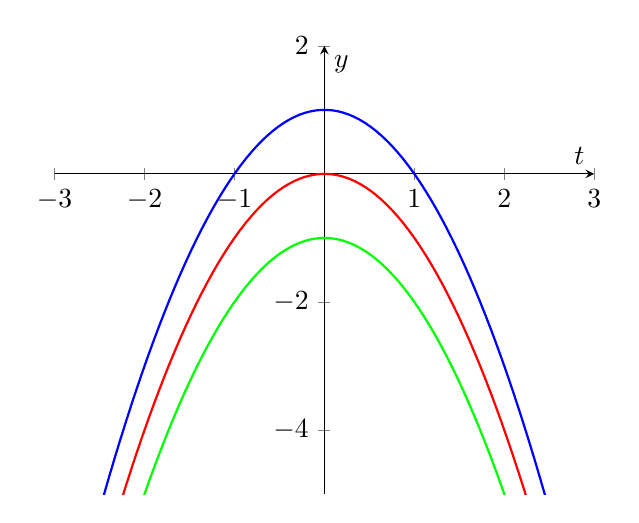
\begin{tikzpicture}
        \begin{axis}[
            axis lines = middle,
            xlabel = \(t\),
            ylabel = \(y\),
            xmin=-3, xmax=3,
            ymin=-5, ymax=2,
            samples=100,
            domain=-3:3
        ]
        \addplot[blue, thick] {1 - x^2} node[above,pos=0.9]{$m=1$};
        \addplot[red, thick] {0 - x^2} node[above,pos=0.9]{$m=0$};
        \addplot[green, thick] {-1 - x^2} node[below,pos=0.9]{$m=-1$};
        \end{axis}
    \end{tikzpicture}
    \caption{Isoclines for slopes $m = -1$, $m = 0$, and $m = 1$}
\end{figure}

\section*{Problem 3}

\subsection*{Part (a)}
\textbf{Problem Statement:} Solve the IVP \( y' = \frac{t^2 + 7}{y^4 - 4y^3} \), \( y(1) = 2 \), and leave the answer in implicit form.

\textbf{Solution:}
This equation can be separated:

\[
(y^4 - 4y^3) \, dy = (t^2 + 7) \, dt
\]

Integrating both sides:

\[
\int (y^4 - 4y^3) \, dy = \int (t^2 + 7) \, dt
\]

The integrals are:

\[
\frac{y^5}{5} - y^4 = \frac{t^3}{3} + 7t + C
\]

Given \( y(1) = 2 \), substitute to solve for \( C \):

\[
\frac{(2)^5}{5} - (2)^4 = \frac{(1)^3}{3} + 7(1) + C
\]

Simplifying:

\[
\frac{32}{5} - 16 = \frac{1}{3} + 7 + C
\]

Solve for \( C \):

\[
    C = -\frac{254}{15}
\]

Thus, the implicit solution is:

\[
\frac{y^5}{5} - y^4 = \frac{t^3}{3} + 7t -\frac{254}{15}
\]

\subsection*{Part (b)}
\textbf{Problem Statement:} Solve \( y' = \cos^2(y) \ln|t| \).

\textbf{Solution:}
Separate the variables:

\[
\frac{1}{\cos^2(y)}dy = \ln|t| \, dt
\]

Integrating both sides:

\[
\int \sec^2(y) \, dy = \int \ln |t| \, dt
\]

\[
\tan(y) = t \ln|t| - t
\]

Thus, the explicit solution is:
\[
\ y = \tan^{-1}(t \ln t - t + C)
\]

\subsection*{Part (c)}
\textbf{Problem Statement:} Solve \( (t^2 + t) y' + y^2 = t y^2 \), with \( y(1) = -1 \).

\textbf{Solution:}
Rewriting the equation:

\[
(t^2 + t) y' = t y^{2} - y^{2} = y^{2} (t - 1)
\]

Separate variables:

\[
\frac{1}{y^{2}}dy = \frac{(t-1)}{(t^{2} + t)} \, dt
\]

Integrating both sides:
\[
\int \frac{1}{y^{2}}dy = \int \frac{(t-1)}{t^{2}+t}
\]

Integration of the right side by partial fractions
\[\int \frac{(t-1)}{t^{2}+t} \\ \]
\begin{align*}
\frac{(t-1)}{t^{2}+t} &= \frac{(t-1)}{t(t+1)} \\
\frac{(t-1)}{t(t+1)} &= \frac{A}{t} + \frac{B}{t+1} \\
\end{align*}

\quad Solve for A and B:
\begin{align*}
t-1 &= A(t+1) + Bt \\  
&= t(A+B) + A \\
A &= -1 \\
B &= 2 \\
\end{align*}

\quad Substitute:
\begin{align*}
\int \frac{(t-1)}{t^{2}+t} &= \int -\frac{1}{t} + \frac{2}{t+1} \\
&= -\ln|t| + 2 \ln|t+1| + C
\end{align*}

Plugging the integral back into the original equation:
\begin{align*}
\int \frac{1}{y^{2}}dy&= \int \frac{(t-1)}{t^{2}+t} \\
-\frac{1}{y} &= -\ln|t| + 2 \ln|t+1| + C
\end{align*}

Solve for C with y(1) = -1
\begin{align*}
-\frac{1}{y}&= -\ln|t| + 2 \ln|t+1| + C \\
-\frac{1}{(-1)}&= -\ln|(1)| + 2 \ln|(1)+1| + C \\
1 &= 0 + 2\ln|2| + C \\
C &= 1 - 2 \ln|2|
\end{align*}

Thus, the explicit solution is:
\[
y = \frac{1}{\ln|t| - 2 \ln|t+1| - 1 + 2 \ln|2|}
\]

\section*{Problem 4}
\textbf{Problem Statement:} Solve given the differential equation: $\frac{dy}{dt} = \frac{2y^4 + t^4}{ty^3}$

\textbf{Solution:} We use the substitution \( v = \frac{y}{t} \), which gives \( y = vt \). Differentiating both sides with respect to \( t \), we obtain:



\[
\frac{dy}{dt} = v + t \frac{dv}{dt}
\]

Substituting this into the original differential equation:

\[
v + t \frac{dv}{dt} = \frac{2(vt)^4 + t^4}{t(vt)^3} = \frac{2v^4t^4 + t^4}{t^4v^3} = \frac{2v^4 + 1}{v^3}
\]

Thus, the equation becomes:

\[
v + t \frac{dv}{dt} = \frac{2v^4 + 1}{v^3}
\]

Rearranging to isolate \( \frac{dv}{dt} \), we get:

\[
\frac{dv}{dt} = \frac{v^4 + 1}{tv^3}
\]

Finally, separating the variables gives:

\[
\frac{v^3}{v^4+1} dv = \frac{dt}{t}
\]

Integrating both sides:

\[
\int \frac{v^3}{v^4+1} dv = \int \frac{dt}{t}
\]

Integration of left side by u-sub with $u = v^4 + 1$ and $dx = 1/v^3$:
\begin{align*}
\int \frac{v^3}{4vu} &= \int \frac{1}{4u} \\
\frac{1}{4} \int \frac{1}{u} &= \frac{1}{4} \ln|u| = \frac{1}{4} \ln|v^4 + 1| \\
\int \frac{v^3}{4vu} &= \frac{1}{4} \ln|v^4 + 1|
\end{align*}

Plugging the integral back into the original equation:
\[
\int \frac{v^3}{v^4+1} dv = \int \frac{dt}{t} \\
\]

Recalling that $v = \frac{y}{t}$, we get the implicit solution:
\[
\frac{1}{4} \ln|(\frac{y}{t})^4 + 1| = \ln|t| + C
\]


\section*{Problem 5}

\textbf{Problem Statement:} Solve the ODE \( y' = (y + t)^2 \) using \( u = y + t \).

\textbf{Solution:}
Substitute \( u = y + t \), so \( y' = u^2 \). The equation becomes:

\[
\frac{du}{dt} = u^2
\]

Because we use the substitution \( u = y + t \) we can rearange to give us \( y = u - t \). Differentiating both sides with respect to \( t \):

\[
\frac{dy}{dt} = \frac{du}{dt} - 1
\]

Substituting into the equation \( y' = (y + t)^2 \):

\begin{align*}
\frac{du}{dt} - 1 &= u^2 \\ 
\frac{du}{dt} &= u^2 + 1
\end{align*}

This is now a separable differential equation. We separate the variables and integrate:

\[
\int \frac{du}{u^2 + 1} = \int dt
\]

Integration of left side by:
\[
\int \frac{1}{a^2 + x^2} dx = \frac{1}{a}tan^{-1}(x/a) + C
\]
\[
\int \frac{du}{u^2 + 1}  = tan^-1(u)
\]

Plugging the integral back into the equation:
\[
\int \frac{du}{u^2 + 1} du = \int dt
\]
\[
tan^{-1}(u) = t + C
\]
Solving for \( u \):

\[
u = \tan(t + C)
\]

Recalling that \( u = y + t \), we substitute back:

\[
y + t = \tan(t + C)
\]

Finally, solving for \( y \):

\[
y = \tan(t + C) - t
\]

Thus, the general solution to the original differential equation is:

\[
y = \tan(t + C) - t
\]
\section*{Problem 6}

\subsection*{Part (a)}
\textbf{Problem Statement:} Express the radius of the raindrop as a function of time.

\textbf{Solution:}
The rate of decrease of the volume is proportional to the surface area. For a sphere, \( V = \frac{4}{3} \pi r^3 \) and \( S = 4 \pi r^2 \). The differential equation is:

\[
\frac{dV}{dt} = -k S
\]

Substitute $S = 4 \pi r^3$ and $V = \frac{4}{3}\pi r^3$

\[
\frac{d(\frac{4}{3}\pi r^3)}{dt} = -4k \pi r^3
\]

Take the derivative of $r$ with respect to $t$

\begin{align*}
4\pi r^3 \frac{dr}{dt} &= -4k \pi r^3\\
r &= -kt + C
\end{align*}

Thus $r$ is a linear fucntion with respct to $t$. We can solve for the unkowns k and c by substituting the intitial conditions $r(0) = 1$ and $r(2) = 1/2$

\begin{align*}
    r &= -kt + C \\
    1 &= -k(0) + C \\
    1 &= C \\
    \\ 
    \frac{1}{2} &= -k(2) +1\\
    \frac{1}{4} &= k
\end{align*}

Thus our final function of r with respect to time is:
\[
r(t) = -\frac{1}{4}t + 1
\]
\subsection*{Part (b)}
\textbf{Problem Statement:} When will the raindrop evaporate completely?

\textbf{Solution:}
Solve for \( t \) when \( r(t) = 0 \).
\begin{align*}
   r(t) &= -\frac{1}{4}t + 1 \\
   0  &= -\frac{1}{4}t + 1 \\
   -1 &= -\frac{1}{4}t \\ 
   4 & = t 
\end{align*}
\section*{Problem 7:}
\textbf{Problem Statement:} Consider the IVP $y' = t\sqrt{t}, y(1) = 4$. Use Euler's Method to determine an estimate to the value of $y(1.5)$ using step sizes of
$h_1 = 0.1$ and $h_2 = 0.05$.

\textbf{Solution:}
\begin{table}[h!]
    \centering
    \pgfplotstableread[col sep=comma]{Euler_Method_Results_Comparison.csv}\loadedtable
    \pgfplotstabletypeset[
        col sep=comma,
        string type,
        every head row/.style={before row=\toprule, after row=\midrule},
        every last row/.style={after row=\bottomrule},
        columns/Step/.style={column name=Step},
        columns/Approximate Value/.style={column name=Approximate Value},
        columns/Exact Value/.style={column name=Exact Value},
        columns/Error/.style={column name=Error}
    ]{\loadedtable}
    \caption{Euler's Method Approximations}
    \label{tab:euler_method}
    \end{table}
Yes. The smaller step size results in a more accurate approximation.
\end{document}
